\documentclass[10pt]{article}
\usepackage{fontspec}
\usepackage{jim}
\usepackage{amsmath}
\usepackage{csquotes}
\usepackage{polyglossia}
\setdefaultlanguage{french} 
\usepackage{listings}
\usepackage{diagbox}
\usepackage{caption}
\usepackage{booktabs}
\usepackage{microtype}
\usepackage{graphicx}
\usepackage{hyperref}
\usepackage{tikz}
\usepackage{xspace}
\usepackage{array}
\usepackage{subcaption}
\usepackage{placeins}
\usepackage[backend=biber]{biblatex}
\usepackage{authblk}
\addbibresource{biblio.bib}

\setmainfont{Times New Roman}
\setmonofont{Fira Code}
\newcolumntype{C}[1]{>{\centering\arraybackslash}m{#1}}   %% centered
\newcolumntype{R}[1]{>{\raggedright\arraybackslash}m{#1}}  %% right aligned
\newcolumntype{L}[1]{>{\raggedleft\arraybackslash}m{#1}}  %% right aligned

\newcommand\timenode{nœud temporel\xspace}
\newcommand\trigger{point d'interaction\xspace}
\newcommand\triggers{points d'interaction\xspace}
\newcommand\ossia{OSSIA\xspace}
\newcommand\vocab[1]{\textbf{#1}}
\DeclareCaptionType{scenario}[\bfseries Scénario]
% Title.
% ------
\title{Exécution répartie de scénarios interactifs}

\author[1,2]{Jean-Michaël Celerier$^*$\thanks{$^*$: jcelerier@u-bordeaux.fr}}
\author[1]{Myriam Desainte-Catherine$^{**}$\thanks{$^{**}$: myriam@labri.fr}}
\author[2]{Jean-Michel Couturier$^{***}$\thanks{$^{***}$: jmc@blueyeti.fr}}
\affil[1]{Univ. Bordeaux, LaBRI, UMR 5800, F-33400 Talence, France}
\affil[2]{ Blue Yeti, F-17110 France}

\renewcommand\Authands{, }

\begin{document}
\maketitle
\begin{abstract}
    La pratique musicale est souvent une opportunité pour interagir et échanger, 
    avant tout avec d'autres musiciens, et plus récemment avec des algorithmes ou logiciels 
    disposant d'un certain degré d'autonomie et de liberté.
    
    La notation musicale occidentale résout le problème du partage et de la séparation d'information entre musiciens 
    en divisant une partition en portées; la plupart des logiciels musicaux vont interpréter ces portées sur une seule machine, en gardant la possibilité de pistes avec des réglages indépendants. 
    
    Ce travail consiste en une généralisation de cette notion de partage aux scénarios interactifs, en permettant une exécution synchrone ou asynchrone de différentes parties d'un même scénario sur plusieurs machines, lors d'une seule exécution.
    
    Une implémentation est offerte dans le logiciel i-score, avec pour objectif de mettre en valeur 
    les nouvelles possibilités d'écriture qu'offre une exécution répartie à un compositeur.
\end{abstract}

\section{Introduction}
On cherche à définir une sémantique permettant de décrire l'exécution d'une partition interactive sur plusieurs machines d'un réseau local, en prenant en compte les exécutions parallèles, c'est-à-dire que deux machines jouent ensemble, de manière synchronisée ou non, ainsi que les exécutions sérielles : une machine joue une partie, puis une autre joue la suite.

On parle ici de « jeu » de manière abstraite~: on s'intéresse au contrôle de tous types de paramètres et non pas uniquement aux paramètres musicaux.

On présentera plusieurs applications et besoins rencontrés par des artistes et auteurs, qui ont motivé ce travail.

À partir de ces besoins, on cherche à définir les ajustements nécessaires au modèle \ossia pour permettre d'exprimer le plus simplement possible des structures réparties dans une partition interactive.

Une des premières questions est la nature de la synchronisation désirée entre les machines.
Par exemple, des choix d'implémentation sont nécessaire en fonction de la précision désirée. 
On s'impose de plus pour ce travail un fonctionnement sur du matériel grand public.

Puis, les possibilités de répartition étudiées seront présentées, en analysant l'impact que peuvent avoir les problèmes connus dans le domaine de l'informatique répartie, sur l'écriture de telles partitions. 
Notamment, on donnera différentes sémantiques possibles pour plusieurs éléments du modèle \ossia, qui permettent de répondre à des cas d'application distincts. 

On considérera le partage d'information qu'il peut y avoir entre machines exécutant une même tâche en parallèle, et les différentes manières de synchroniser ces machines entre elles.

Pour conclure, les détails d'une première implémentation seront présentés.

%TODO notation graphique pour groupes, synchrone, asynchrone, etc... ?
\section{Études de cas}

\subsection{Projet Quarrè}

\begin{figure}[h]
    \centering
    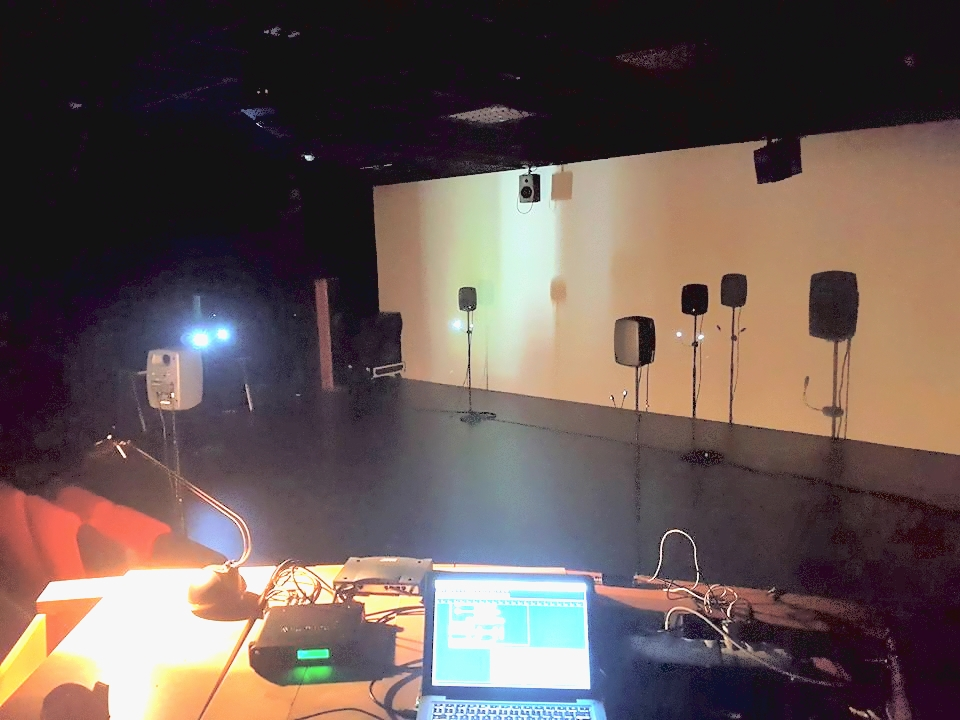
\includegraphics[scale=0.2]{images/quarre.jpg}
    \caption[Quarrè]{Quarrè sans participants. Pierre Cochard, 2016.}
    \label{img.quarre}
\end{figure}

Quarrè
\footnote{\tiny\url{https://scrime.labri.fr/blog/quarre-composition-interactive}} est une installation interactive en son spatialisé réalisée par Pierre Cochard au SCRIME. 
Elle utilise Max/MSP, i-score, et une application mobile développée pour l'occasion. 
Elle implique entre un et cinq participants possédant chacun un téléphone.

Une trame principale d'environ une demi-heure se déroule sur une machine fixe.
Durant cette trame, à différents moments, les participants vont pouvoir interagir via l'application mobile. 
Les actions possibles varient en fonction du nombre de participants présents lors de chaque représentation.
L'application les avertit par un compte à rebours de la date de leur prochaine interaction. 
Ils disposent ensuite d'une durée déterminée pour agir : changer un paramètre d'un effet, déclencher des sons, spatialiser un objet sonore\dots{}
Par exemple, entre $t=1m30$ et $t=2m$, deux des participants vont pouvoir changer l'intensité d'un effet de chorus, et deux autres vont pouvoir déplacer un objet sonore dans la scène spatiale. 

Ce projet permet d'exhiber plusieurs besoins importants : 
\begin{itemize}
    \item La présence d'une forme de polyphonie répartie, avec un nombre de « voix » non fixées au moment de l'écriture.
    \item L'écriture de cette polyphonie dans le temps : à un instant, au plus deux téléphones sont actifs, à  un autre instant aucun ne l'est, etc.
    \item Le fonctionnement sur des réseaux avec des caractéristiques non idéales, comme le réseau WiFi des téléphones mobiles.
\end{itemize}
%- Cas des applis de téléphone : un objet qui s'exécute sur plusieurs machines en parallèle (dont on veut aggréger les résultats)

\subsection{Besoins additionnels}
\subsubsection{Support des périphériques embarqués}
Actuellement, une des manières principales d'utiliser le logiciel i-score est de lui faire faire du contrôle par réseau. 

Néanmoins, pour des applications embarquées, par exemple sur Raspberry Pi, cela peut avoir les conséquences suivantes~: 
\begin{itemize}
    \item Encombrement de la bande passante : certains périphériques ne sont pas en Gigabit Ethernet; envoyer des quantités importantes de messages OSC sur des intervalles de quelques millisecondes va entraîner des pertes de paquets, des retards, et une augmentation de la latence.
    \item Gigue\footnote{De l'anglais \textit{jitter}} sur les messages envoyés qui peut entraîner des effets indésirables comme des tremblements si par exemple on fait se déplacer des objets graphiques par réseau.
    \item Consommation superflue de ressources pour le décodage des messages réseaux.
\end{itemize}

%De plus, actuellement, il est nécessaire de copier les fichiers de sauvegarde sur le périphérique à chaque modification que l'on veut tester, ce qui est peu ergonomique. 
%Le système devra donc permettre de partager automatiquement un scénario entre deux machines.

\subsubsection{Lecture de médias synchronisée}
On désire offrir des possibilités de lecture permettant à 
des clips audio ou vidéo de démarrer au même instant sur plusieurs machines, 
puis de rester synchronisés durant la lecture.

Par exemple, un mur de vidéos synchronisées basé sur de l'embarqué, avec 
une évolution interactive des vidéos projetées : lorsqu'une personne rentre dans la salle, une vidéo se met à jouer sur tous les écrans ; cette vidéo change à chaque fois qu'une personne sort.

Il est important pour des raisons artistiques que la synchronisation temporelle soit très forte entre les différentes machines : quelques dizaines de millisecondes de décalage entre deux vidéos peuvent déjà être perturbantes pour le public. 
Le problème est encore plus prononcé avec de l'audio.

\subsubsection{Redondance}
Le matériel n'étant pas infaillible, la question de la tolérance aux pannes se pose~: comment mitiger une panne de l'ordinateur principal pendant une représentation artistique ?

Une des possibilités est d'offrir un système de redondance : si une machine tombe en panne, une autre prend le relais le plus vite possible.
La machine prenant le relai doit donc avoir été maintenue en synchronisation avec la machine étant tombé en panne, pour garantir le moins de perturbations possibles lors de la bascule.
 
%- Donner la possibilité de faire un dialogue (boucle avec un coup un \trigger qui vient de A, un coup un \trigger qui vient de B, etc)
%- Approche alternative avec application mobile.

\section{État de l'art}
\subsection{Musique répartie}
Il existe plusieurs familles de logiciels et outils offrant un fonctionnement en réseau pour la production musicale.
On distingue notamment les applications ayant pour but de synchroniser des 
flux audio sur plusieurs machines, des applications permettant une collaboration lors 
de l'écriture et de la composition musicale.

Dans le premier cas, on notera principalement les multiples incarnations de NetJack\cite{carot2009netjack}, 
ayant pour but de rendre accessible les éléments d'une baie de raccordement Jack sur plusieurs machines. 
Ce sont des extensions maître-esclave de Jack qui permettent à une machine d'envoyer un flux audio ou MIDI sur une autre en branchant un câble virtuel.
Un recensement plus complet des serveurs de son distribués ayant pour but les performances musicales en réseau est donné dans~\cite{carot2007networked}. 

Différents logiciels permettant une écriture collaborative, mais non synchronisée, existent : 
Ohm Studio\cite{koszolko2015crowdsourcing} reprend le principe des séquenceurs traditionnels et permet un partage de document à plusieurs utilisateurs, sur internet.
Splice\cite{pignato2015deterritorialized} suit le même principe, mais est orienté vers la communauté des \emph{beat-makers}.

Enfin, il existe une famille importante d'outils orientés vers l'improvisation musicale répartie en temps réel\cite{mills2010dislocated}. 
On citera notamment NINJAM\footnote{\url{http://ninjam.com}} et eJamming\footnote{\url{http://www.ejamming.com/}}.

%\subsubsection{Lien entre la répartition à l'édition et la répartition à l'exécution}

\subsection{Horloges}
En raison de la nature temporelle du problème présenté, on s'intéresse aux mécanismes possibles pour la gestion du temps entre plusieurs machines.

La littérature sur les systèmes distribués distingue plusieurs familles d'horloges : 
\begin{itemize}
    \item Les horloges physiques marquent l'avancement du temps dans le monde matériel.
    \item Les horloges logiques marquent l'avancement du temps dans les étapes d'un algorithme réparti, donc sans relation avec du temps en secondes.
    \item Plus récemment, les horloges hybrides ont été introduites afin de concilier ces deux familles.
\end{itemize}

Les deux principales méthodes pour la synchronisation d'horloges physiques sont \emph{Network Time Protocol}\cite{mills1991internet} et \emph{Precision Time Protocol}\cite{peng2009research}. 
Le premier est disponible sur de nombreuses plate-formes et permet en pratique d'atteindre une précision de synchronisation de quelques milliseconde sur internet. 
Le second est plus précis et promet une précision proche de la microseconde. 
Cependant, cela dépend de la précision avec laquelle les paquets sont estampillés\footnote{timestamped} et donc de la qualité de l'horloge de l'implémentation PTP. 
En pratique, l'intérêt de PTP sera plus prononcé lorsque du matériel dédié et onéreux (\emph{Grand Master Clock}) est disponible pour réaliser l'estampillage des paquets.

On rappelle qu'une horloge monotone a pour caractéristique de toujours progresser vers l'avant. 
Un des désavantages de l'utilisation des horloges physiques pour l'estampillage est qu'elles ne sont pas monotones. 
Notamment, les secondes intercalaires bouleversent régulièrement les systèmes distribués basés sur les horloges physiques.

Les horloges logiques ont été introduites par Leslie Lamport~\cite{lamport1978time} afin d'offrir des possibilités de raisonnement et de vérification formelles sur l'écoulement du temps dans les systèmes répartis.
Notamment, les estampilles de Lamport permettent d'offrir un ordre partiel entre les messages échangés dans un système réparti.

Ce mécanisme a été par la suite généralisé, d'abord par les horloges vectorielles, puis par les horloges matricielles. 
Dans le premier cas, chaque message contient un tableau contenant l'horloge de son émetteur ainsi que les horloges connues des autres processus. Dans le second cas, chaque message contient le vecteur contenant les vecteurs d'horloges de chaque processus.

Des solutions existent pour maintenir un lien entre les horloges logiques et physiques. 
Par exemple, Google a introduit TrueTime dans le cadre de la base de données distribuée Spanner\cite{corbett2013spanner}. 
TrueTime travaille avec des intervalles plutôt que des dates précises, et requiert une synchronisation très précise des horloges physiques, utilisant des signaux GPS et des horloges atomiques.

Les horloges logiques \textit{hybrides}\cite{kulkarni2014logical} offrent des garanties de causalités sur une horloge physique proche de la précision de NTP, avec une granularité proche de la microseconde.

Enfin, pour les musiciens, des horloges basées non pas sur un temps en secondes, mais sur un temps musical ont été présentées récemment. Elles permettent de s'assurer que plusieurs machines vont jouer sur un même \textit{beat}. C'est le cas par exemple avec Ableton Link\footnote{\url{https://www.ableton.com/en/link/}}. 
On notera aussi le Métronome Global\cite{oda2016global}, qui utilise des Raspberry Pi et une connection GPS pour offrir ce genre de synchronisation.

%Problème de l'horloge : 
%\begin{itemize}
%\item Si on utilise l'horloge système, pas de garantie qu'elle soit bien synchronisée. 
%Et NTP pas dispo partout (on n'a pas forcément les droits sur un téléphone pour changer l'heure).
%Horloge i-score se resynchronise déjà en cas de délai sur une machine.
%\item Si on utilise une horloge interne, problème de la synchronisation avec l'horloge système (pour le tick)
%\end{itemize}
%\url{http://www.cse.buffalo.edu/tech-reports/2014-04.pdf}
%\url{http://queue.acm.org/detail.cfm?id=2745385}
%\url{http://radar.oreilly.com/2012/10/google-spanner-relational-database.html}
%\url{http://www.ntp.org/ntpfaq/NTP-s-sw-clocks-quality.htm}
%\url{https://en.wikipedia.org/wiki/Synchronous_Ethernet}a
%\url{https://en.wikipedia.org/wiki/Time_and_frequency_transfer}
%\url{http://vlsicad.ucsd.edu/courses/ece260b-w07/papers/clock/Friedman.pdf}
%\url{http://www.ceu-lang.org/try.php}
%\url{https://zookeeper.apache.org/}

%Faire la relation entre notre système et le problème CAP : \url{https://en.wikipedia.org/wiki/PACELC_theorem}

%Horloges logiques : équivalent à envoyer une timestamp à chaque tick (on arrive donc à un méchanisme de vector clock approximatif). 

%Synchro d'horloges de deux clionts dont une qui ralenti, si elles exécutent le même  scénario ? Il faut les recaler régulièrement. 

%Possibilité : externe (NTP, etc) ou interne : \url{https://github.com/ethanlim/NetworkTimeProtocol}

%Recaler dès qu'on accumule du retard ?

%On peut introduire un recalage sur la master clock entre chaque tick.

% Ce qu'on fait : ping régulier vers chaque client (toutes les 100 millisecondes)

% Quand quelque chose doit se synchroniser, on dit à chaque client à quel instant il est supposé arriver par rapport à son horloge système.

% Quand un client reçoit un ordre pour un timenode à t, il l'applique dès que t <= local(t) (modulo un tick?)

% Possibilité : synchronisation via démon externe (PTP, NTP...), mais pas toujours possible (on ne peut pas supposer que l'utilisateur a les droits pour changer l'horloge sur sa machine).

% Synchronous ethernet

% Ableton Link : synchro sur les ticks musicaux 

% Avoir une horloge propre à i-score ? Mais du coup maintenant il faut la synchroniser à l'horloge système. 

%\subsubsection{Problématique de la sécurité}
%On veut : résistance aux "normal" failures, pas Byzantine failures.

% \subsubsection{Synchronisation de médias}
% - pas pour l'instant... doivent être au même endroit sur la même machine.
% Ableton Link ? Netjack ?

\section{Approche}
Cette section détaille les choix de haut niveau réalisés.

On souhaite modifier le moins possible le modèle \ossia, 
en rajoutant les notions nécessaires et suffisantes pour offrir la finesse de répartition désirée.

La section~\ref{sec.description} présente de manière détaillée les possibilités 
de répartition offertes, en prenant exemple sur des cas simples.

La section~\ref{sec.semantique} définit ces possibilités en utilisant les objets du modèle \ossia. 
On notera que cette méthode serait prohibitive à réaliser manuellement par le compositeur~: c'est un guide pour réaliser l'implémentation. 
La répartition se fait automatiquement à partir de la spécification de haut niveau que donne le compositeur via les outils présentés en section~\ref{sec.description}. 

% TODO REVIEW THIS SENTENCE
On prendra garde à ne pas confondre ce travail avec la forme de répartition qui existe déjà dans le projet et permet d'orchestrer d'autres logiciels via des protocoles comme OSC.

% Enfin, la section~\ref{sec.implementation} présente une évaluation des performances dans le cadre d'une implémentation pratique.

%-------------------------------------------
%Première approche basées sur réseau de Pe-tri.

%Puis migration du modèle d'i-score maintenant autonome.


%- Problème des devices. Note : si on se permet d'envoyer des messages OSC quelconques (i.e. pas dans l'arbre), ça peut simplifier des choses. Aussi, permettre devices qui sont juste en mode envoi ? Il faut un autre proto que OSC ou Minuit...

%Aussi, refactoriser pour utiliser tout i-score en librairie

%Différentes possibilités de répartition sont disponibles selon les types de processus.

%Détailler les implications des choix par rapport au théorême CAP et PACELT.

\subsection{Rappel du modèle}
On s'intéresse à la problématique de répartition dans le cadre du logiciel i-score, qui implémente le modèle \ossia\cite{celerier2015ossia} pour les partitions interactives.
Il consiste en un agencement d'éléments permettant de définir des comportements temporels. 
Les éléments dont nous avons besoin ici sont : 
\begin{itemize}
	\item \vocab{Contrainte temporelle} : décrit un écoulement de temps. 
    Représenté par un trait horizontal. 
	\item \vocab{Nœud temporel} : synchronise le début et la fin de plusieurs contraintes temporelles. Représenté par un trait vertical.
	Peut porter un \vocab{point d'interaction}, qui décrit l'attente et la résolution d'une condition externe pour stopper les contraintes précédentes et démarrer les suivantes; les contraintes précédentes seront alors en partie représentées par des pointillés pour exprimer l'incertitude sur leur date de fin. 
    Cette incertitude peut être bornée par des dates d'exécution minimales et maximales.
    La condition prend la forme d'une expression logique entre paramètres de la partition. Par exemple, 
    
    \lstinline|/couleur == "rouge" && /volume > 1| .
	\item \vocab{Processus} : contenu dans les contraintes temporelles, permet l'exécution d'un comportement à chaque tic d'horloge. Par exemple, une automation.
	\item \vocab{État} : permet d'envoyer un message à un temps donné. Représenté par un point.
\end{itemize}
Des exemples sont visibles en section~\ref{sec.description}, par exemple les scénarios~\ref{scenar.hierarchy} et~\ref{scenar.general}.
%\subsubsection{Répartition à l'édition}

\subsection{Nouvelles notions}
Nous nous trouvons en présence de plusieurs ordinateurs qui communiquent et partagent une même structure de donnée : un document.
L'ensemble constitué par les instances d'i-score et le document qu'elles partagent est appelé \vocab{session}.

On désigne par \vocab{client} une instance d'i-score connectée à une session, qui peut être sur une machine différente.

On désire s'affranchir des notions propres aux machines physiques et des problématiques de réseau, telles que adresses IP, ports des machines, lors de l'écriture d'un scénario réparti. 

Pour ce faire, la notion de \vocab{groupe} est introduite. 
Un groupe est un ensemble de clients auxquels les mêmes objectifs d'exécution sont assignés.
Les compositeurs ne manipulent jamais directement les informations relatives à un client, uniquement celle d'un groupe qui peut contenir zéro, un, ou plusieurs clients.

De manière générale, quand plusieurs clients font partie d'un même groupe, cela signifie qu'ils vont réaliser les mêmes tâches, à des degrés de synchronisation variables.

Un des intérêts de cette approche est la tolérance aux pannes, déconnections, reconnections, et changements d'installation. 
Par exemple, si une machine tombe en panne, il est possible de la remplacer par une autre simplement en l'assignant au même groupe que la machine en panne 
sans avoir besoin de mettre à jour le scénario.


\begin{figure}[h]
	\centering
	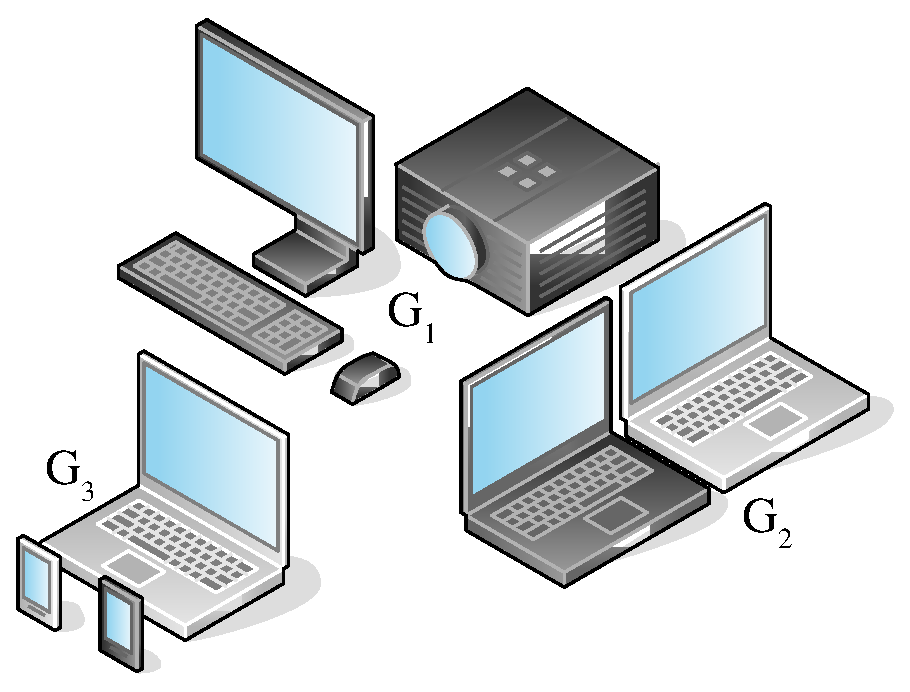
\includegraphics[scale=0.4]{images/groupes.eps}
	\caption{Plusieurs groupes $G_1,G_2,G_3$ avec plusieurs groupes hétérogènes.}
	\label{img.groupes}
\end{figure}


\section{Description de l'exécution}\label{sec.description}
On sépare les objets offrant une structure temporelle, des objets possédant des données et commandes envoyées à d'autres logiciels (par exemple, une automation).

Des groupes et des spécifications de synchronisation sont assignées à ces objets par le compositeur; en pratique, ces informations sont enregistrées comme une liste de méta-données associées aux objets.
% Il est possible d'assigner plusieurs groupes à un objet; cela se comporte comme un groupe constitué de la somme des clients de chaque groupe était assigné.

% *** est-ce que ce n'est pas plus intéressant d'essayer de spécifier le cas ou on a plusieurs groupes sur plusieurs objets ? 

\subsection{Processus de contenu}
On entend par processus de contenu, tous les processus produisant des données, sans se soucier de la structure temporelle. 
En voici une liste non exhaustive : automation, mapping, code javascript, piano-roll MIDI, lecture de son\dots

Le processus s'exécute tel quel pour tous les clients auquel il est assigné, 
et ne s'exécute pas pour les autres.

Ici les processus de contenu sont représentés par une boite barrée en diagonale, qui représente le cas courant d'une automation montante.
% TODO pour devices, faire en sorte que les clients ne se connectent que à ceux qui sont en local ? Ou même mode "non connecté" (mais impossible de recevoir comme ça). Ou bien avoir une "map" d'addresse ip / port pour chaque paire client <-> device.

\subsection{Processus Scénario}
Le scénario est le processus central d'i-score : il met en relation les différents éléments temporels, en parallèle et en série.

Plusieurs manières de répartir l'exécution d'un scénario, offrant différentes possibilités d'écriture, sont détaillées ci-dessous. 
On sépare le cas général permettant l'interactivité dans un scénario du cas plus simple ou les dates sont fixées.
Dans le premier cas (scénario~\ref{scenar.general}), l'avancement dépend du déclenchement d'un évènement externe, tandis que dans le second (scénario~\ref{scenar.non-interactif}), l'avancement ne dépend pas de paramètres externes. 

On travaillera dans les exemples suivants avec plusieurs groupes $G_{1\dots N}$ disposant chacun d'un nombre inconnu de clients. 
On pourra supposer que les contraintes temporelles portent chacune des processus de contenus, qui ne sont pas toujours représentés ici afin de garder les figures simples.

Dans le modèle \ossia, le nœud temporel est l'objet permettant de synchroniser le début et la fin de plusieurs structures temporelles. 
Nous analysons d'abord les choix qui doivent être fait pour traduire ce mécanisme dans le cas réparti, puis étudions l'impact sur le processus scénario dans son ensemble en présentant les politiques de répartition de haut niveau.
\subsubsection{Modes de synchronisation}
Il est difficile d'offrir une synchronisation forte (par exemple avec une précision d'une milliseconde, dans un système réparti\cite{sheehy2015there}. 
Une contrainte additionnelle que l'on s'impose est le fonctionnement du système sur du matériel grand public. 
Ce matériel ne supportera pas toujours des fonctionnalités telles que Ethernet synchrone\cite{ferrant2008synchronous} ou PTP.

%NOTE : il faut changer les noms. Asynchrone / Simultané => Instantané / Compensé et Ordonné / Non-ordonné => Synchrone / Asynchrone

On identifie deux possibilités de synchronisation, manifestant leur utilité dans des cas différent : 
\begin{itemize}
	\item Mode synchrone : respecte la sémantique \ossia{}~: les éléments s'exécutent dans le même ordre que si le scénario n'était pas réparti, au prix d'une latence augmentée en présence d'interactivité.
	\item Mode asynchrone : ne respecte pas la sémantique~: une exécution d'un objet peut terminer après que l'exécution de l'objet suivant ait commencé. En revanche, la latence est diminuée.    
\end{itemize}

De plus, on considère la manière dont l'information se propage dans le système :

\begin{itemize}
	\item Propagation instantanée : lorsqu'une information interactive est disponible dans le système (par exemple «une expression se vérifie»), elle est propagée le plus vite possible aux autres clients qui doivent appliquer le résultat de cette information. 
    Ce mode permet de réduire la latence, au prix de décalages plus importants entre différents clients.
	\item Propagation compensée : lorsqu'une information est disponible dans le système, elle est propagée de manière à ce que la date absolue de réalisation soit la même (pour un observateur externe) pour tous les clients. 
	On prend en compte pour ce faire les horloges et la latence relative de chaque client~; les dates fixées sont compensées par rapport à cette information.
	C'est utile notamment dans le cas non-interactif : dès qu'une date peut être fixée, elle l'est, et les clients n'attendent pas de message annonçant la fin. 
	Il convient de rappeler qu'il est physiquement impossible d'exécuter les objets avec la même précision temporelle que s'ils étaient exécutés dans un même tic d'horloge sur le même client~; l'objectif est de minimiser ces décalages temporels.
\end{itemize}

Les quatre modes possibles permettent de faire des choix à l'écriture en fonction des besoins en terme de consistance et de latence.

Le mode asynchrone instantané va offrir les plus basses latences au détriment de l'ordre d'exécution des objets.
Inversement, le mode synchrone compensé permet d'offrir une synchronisation forte qui peut être utile pour des processus média. 
On aurait par exemple tendance à choisir ce mode pour démarrer des lectures de vidéo synchronisées sur plusieurs machines.

Les différents modes de synchronisation vont impacter : 
\begin{itemize}
    \item L'exécution des \triggers.
    \item La vérification de la validité des conditions.
    \item Le changement de la vitesse des contraintes temporelles.
\end{itemize}

Lorsqu'un choix doit être fait, un consensus peut être pris au niveau du groupe auquel est assigné l'objet. 
Par exemple, quelle va être la vitesse à laquelle une contrainte temporelle va s'exécuter.
Les mécanismes de consensus possibles sont par la suite discutés en section~\ref{section.consensus}.

\subsubsection{Cas interactif}
On dénote trois manières de partager l'information dans un scénario : 

\begin{itemize}
    \item Aucun partage : Les clients associés à ce processus l'exécutent tous de manière indépendante.
    Les autres ne l'exécutent pas. 
    Si par exemple on assigne le groupe $G_1$ au scénario~\ref{scenar.general}, tous les clients de $G_1$ vont exécuter toutes les contraintes temporelles et évaluer toutes les expressions, sans communiquer entre eux sur leurs résultats. 
    Par exemple, pour deux clients de $G_1$, le \trigger pourra se déclencher à des instants différents, et la condition pourra avoir une valeur différente.
    
    Dans ce cas, les annotations de groupes assignés aux objets du scénario sont récursivement ignorés. 
    Puisque chaque exécution va avoir des temps d'exécution différents pour chaque point d'interaction, il ne peut pas y avoir de synchronisation.
    La seule politique d'exécution qui pourrait faire sens serait que le premier client à valider un \trigger dans un scénario non partagé avertirait les clients suivants.
    
    Ce cas est utile pour des sous-scénarios dont plusieurs participants à une installation artistique font une expérience partagée, tout en gardant une trame générale de plus haut niveau. 
    Typiquement, on peut imaginer ce cas pour une application mobile.
    
    \begin{figure}[h]
        \centering
        \begin{tikzpicture}
        \fill (0, 18.7148) circle (0.075) ; % State.0 
\fill (2.15596, 18.7148) circle (0.075) ; % State.1 
\fill (2.15596, 17.4029) circle (0.075) ; % State.2 
\fill (4.40367, 17.4029) circle (0.075) ; % State.3 
\fill (0, 18.0053) circle (0.075) ; % State.4 
\fill (2.15596, 18.0187) circle (0.075) ; % State.5 
\fill (2.15596, 16.7068) circle (0.075) ; % State.6 
\fill (5, 16.7068) circle (0.075) ; % State.7 
\draw[line width=1pt] (0, 18.7148)  -- (0, 18.0053) ; % TimeNode.0 
\draw[line width=1pt] (2.15596, 18.7148)  -- (2.15596, 16.7068) ; % numb47vine94 
\draw[line width=1pt] (4.40367, 17.4029)  -- (4.40367, 17.4029) ; % faze44greg1 
\draw[line width=1pt] (5, 16.7068)  -- (5, 16.7068) ; % burp79lawn67 
\draw[line width=1pt] (0, 18.7148)  -- (1.39908, 18.7148) ; % dido10rend91 
\draw[dashed,line width=1pt] (1.39908, 18.7148)  -- (2.86239, 18.7148) ; % dido10rend91 
\draw[line width=0.7pt] (1.63908, 18.8678) arc(90:270:0.15) ; % dido10rend91 
\draw[line width=0.7pt] (2.71239, 18.5648) arc(-90:90:0.15) ; % dido10rend91 
\draw (1.07798, 18.9148) node {$A_1$}; % dido10rend91 
\draw[line width=1pt] (2.15596, 17.4029)  -- (4.40367, 17.4029) ; % taut8hews94 
\draw (3.27982, 17.6029) node {$A_2$}; % taut8hews94 
\draw[line width=1pt] (0, 18.0053)  -- (1.38073, 18.0053) ; % ramp48lust85 
\draw[dashed,line width=1pt] (1.38073, 18.0053)  -- (2.90826, 18.0053) ; % ramp48lust85 
\draw[line width=0.7pt] (1.62073, 18.1583) arc(90:270:0.15) ; % ramp48lust85 
\draw[line width=0.7pt] (2.75826, 17.8553) arc(-90:90:0.15) ; % ramp48lust85 
\draw (1.07798, 18.2053) node {$A_3$}; % ramp48lust85 
\draw[line width=1pt] (2.15596, 16.7068)  -- (5, 16.7068) ; % dirt50gage22 
\draw (3.57798, 16.9068) node {$A_4$}; % dirt50gage22 
\draw[line width=1pt] (1.95596, 16.7068)  -- (1.95596, 16.7068) ; % sill78hues28 
\draw[line width=1pt] (1.95596, 16.7068) arc(180:75:0.2) ; % sill78hues28 
\draw[line width=1pt] (1.95596, 16.7068) arc(180:285:0.2) ; % sill78hues28 

        \end{tikzpicture}
        \captionof{scenario}{Un scénario interactif avec des interactions et des conditions ; $G_{1\dots5}$ sont les groupes associés aux éléments du modèle. On suppose l'existence de processus de contenus dans chaque contrainte temporelle.}
        \label{scenar.general}
    \end{figure}
    
    \item Partage complet : il n'y a qu'une seule ligne temporelle commune à tous les clients. 
    Les annotations de groupes indiquent l'emplacement d'exécution des processus de contenu et la liste des clients devant parvenir à un consensus pour une expression donnée. 
    Si par exemple la vitesse d'exécution d'une contrainte est modifiée en temps réel, cette modification est répercutée sur tous les clients.
    
    Cela permet notamment de gérer la répartition d'objets à des niveaux hiérarchiques différents~: dans le scénario~\ref{scenar.hierarchy}, si le scénario racine est dans ce mode, alors on peut correctement faire exécuter les scénarios enfants en prenant en compte les groupes de leurs objets. 
    
    \begin{figure}[h]
        \centering
        \begin{tabular}{L{3.5em}R{0.3\textwidth}}
            Racine: & \begin{tikzpicture}
            \fill (0, 2.20767) circle (0.075) ; % State.1 
\fill (2.23529, 2.20767) circle (0.075) ; % State.2 
\fill (5, 2.20767) circle (0.075) ; % State.3 
\draw[line width=1pt] (0, 2.23364)  -- (0, 2.20767) ; % TimeNode.0 
\draw[line width=1pt] (2.23529, 2.20767)  -- (2.23529, 2.20767) ; % nook18bout42 
\draw[line width=1pt] (5, 2.20767)  -- (5, 2.20767) ; % nato89loop85 
\draw[line width=1pt] (0, 2.20767)  -- (2.23529, 2.20767) ; % step8duct27 
\draw (1.11765, 2.40767) node {$G_1$}; % step8duct27 
\draw[line width=1pt] (0, 2.10767)  -- (2.23529, 2.10767)  -- (2.23529, 1.10767)  -- (0, 1.10767)  -- (0, 2.10767) ;
\draw (1.11765, 1.60767) node {}; % S_1 
\draw[line width=1pt] (2.23529, 2.20767)  -- (5, 2.20767) ; % what68step1 
\draw (3.61765, 2.40767) node {$G_2$}; % what68step1 
\draw[line width=1pt] (2.23529, 2.10767)  -- (5, 2.10767)  -- (5, 1.10767)  -- (2.23529, 1.10767)  -- (2.23529, 2.10767) ;
\draw (3.61765, 1.60767) node {}; % S_2 

            \end{tikzpicture} \\
            $S_1$: & \begin{tikzpicture}[scale=0.4, every node/.style={scale=0.6}]
            
\fill (0, 9.28641) circle (0.075) ; % State.1 
\fill (2.25694, 9.28641) circle (0.075) ; % State.2 
\fill (2.25694, 8.97129) circle (0.075) ; % State.3 
\fill (5, 8.97129) circle (0.075) ; % State.4 
\draw[line width=1pt] (2.25694, 9.28641)  -- (2.25694, 8.97129) ; % loge35long20 
\draw[line width=1pt] (5, 8.97129)  -- (5, 8.97129) ; % wire36tick25 
\draw[line width=1pt] (0, 9.28641)  -- (2.25694, 9.28641) ; % sack65taft69 
\draw (1.12847, 9.8) node {$G_1$}; % sack65taft69 
\draw[line width=1pt] (2.25694, 8.97129)  -- (5, 8.97129) ; % loon80rink81 
\draw (3.62847, 9.5) node {$G_2$}; % loon80rink81 

            \end{tikzpicture} \\
            $S_2$: & \begin{tikzpicture}[scale=0.6, every node/.style={scale=0.6}]
            \fill (0, 9.56564) circle (0.075) ; % State.0 
\fill (1.72897, 9.56564) circle (0.075) ; % State.1 
\fill (1.72897, 9.08927) circle (0.075) ; % State.2 
\fill (3.24766, 9.08927) circle (0.075) ; % State.3 
\fill (3.24766, 9.55873) circle (0.075) ; % State.4 
\fill (5, 9.55873) circle (0.075) ; % State.5 
\draw[line width=1pt] (0, 9.56564)  -- (0, 9.56564) ; % TimeNode.0 
\draw[line width=1pt] (1.72897, 9.56564)  -- (1.72897, 9.08927) ; % jogs95rang7 
\draw[line width=1pt] (3.24766, 9.55873)  -- (3.24766, 9.08927) ; % haul29dade96 
\draw[line width=1pt] (5, 9.55873)  -- (5, 9.55873) ; % vane42mets16 
\draw[line width=1pt] (0, 9.56564)  -- (1.72897, 9.56564) ; % scum85toss49 
\draw (0.864486, 9.76564) node {$G_2$}; % scum85toss49 
\draw[line width=1pt] (1.72897, 9.08927)  -- (3.24766, 9.08927) ; % woof52dyad40 
\draw (2.48832, 9.28927) node {$G_1$}; % woof52dyad40 
\draw[line width=1pt] (3.24766, 9.55873)  -- (5, 9.55873) ; % eben10crux7 
\draw (4.12383, 9.75873) node {$G_2$}; % eben10crux7 

            \end{tikzpicture} \\
        \end{tabular}
        \captionof{scenario}{Deux contraintes possédant chacune un scénario hiérarchique}
        \label{scenar.hierarchy}
    \end{figure}
    
    \item Mixte : il peut y avoir plusieurs lignes temporelles appartenant à différents groupes dans un même scénario. 
    Ces lignes peuvent ensuite se resynchroniser à un instant donné. 
    
    On considère le graphe dont les nœuds temporels sont les sommets et les contraintes temporelles sont les arêtes.
    Les lignes temporelles sont les sous-graphe connexes de ce graphe, telles que les contraintes et les nœuds soient associés au même groupe.
    
    Les annotations donnent l'emplacement d'exécution des contraintes, des processus, et de vérification des expressions. 
%    Un client ne sait pas à l'avance si il va pouvoir se déclencher ou non. 
    
    Considérons le scénario~\ref{scenar.twobranches}. 
    La différence avec le cas du partage complet tient dans le fait que seuls les clients appartenant au groupe $G_1$ vont exécuter la branche du haut.
    Ils peuvent ou non avoir l'obligation de se synchroniser entre eux. 
    L'important est qu'une synchronisation ait lieu pour tous les clients appartenant à $G_1$ et $G_2$ lors du dernier \trigger, situé à droite.
    
    Comme pour le premier cas, en raison de possibilités d'exécutions divergentes du même contenu, il est impossible d'offrir une répartition hiérarchique cohérente.
    
    \begin{figure}[h]
        \centering
        \begin{tikzpicture}
        \fill (0, 23.4797) circle (0.075) ; % State.0 
\fill (1.89189, 23.4797) circle (0.075) ; % State.1 
\fill (1.89189, 22.6223) circle (0.075) ; % State.2 
\fill (5, 22.6223) circle (0.075) ; % State.3 
\fill (5, 20.554) circle (0.075) ; % State.4 
\fill (0, 21.5397) circle (0.075) ; % State.5 
\fill (3.0888, 21.5397) circle (0.075) ; % State.6 
\fill (3.0888, 20.554) circle (0.075) ; % State.7 
\draw[line width=1pt] (0, 23.4797)  -- (0, 21.5397) ; % TimeNode.0 
\draw[line width=1pt] (1.89189, 23.4797)  -- (1.89189, 22.6223) ; % mars98ohio60 
\draw (1.89189, 23.7297) node {$A$}; % mars98ohio60 
\draw[line width=1pt] (5, 22.6223)  -- (5, 20.554) ; % mien5jeer62 
\draw (5, 22.8723) node {$A$}; % mien5jeer62 
\draw[line width=1pt] (3.0888, 21.5397)  -- (3.0888, 20.554) ; % goff74kudo56 
\draw (3.0888, 21.7897) node {$B$}; % goff74kudo56 
\draw[dashed,line width=1pt] (0, 23.4797)  -- (1.89189, 23.4797) ; % gull16loin70 
\draw (0.945946, 23.6797) node {$A$}; % gull16loin70 
\draw[line width=1pt] (1.89189, 22.6223)  -- (4.18919, 22.6223) ; % hits82viva90 
\draw[dashed,line width=1pt] (4.18919, 22.6223)  -- (5, 22.6223) ; % hits82viva90 
\draw[line width=0.7pt] (4.42919, 22.7753) arc(90:270:0.15) ; % hits82viva90 
\draw (3.44595, 22.8223) node {$A$}; % hits82viva90 
\draw[dashed,line width=1pt] (0, 21.5397)  -- (3.0888, 21.5397) ; % drop40disk64 
\draw (1.5444, 21.7397) node {$B$}; % drop40disk64 
\draw[line width=1pt] (3.0888, 20.554)  -- (4.32432, 20.554) ; % jack65dais78 
\draw[dashed,line width=1pt] (4.32432, 20.554)  -- (5, 20.554) ; % jack65dais78 
\draw[line width=0.7pt] (4.56432, 20.707) arc(90:270:0.15) ; % jack65dais78 
\draw (4.0444, 20.754) node {$B$}; % jack65dais78 

        \end{tikzpicture}
        \captionof{scenario}{Deux branches exécutées chacunes par un groupe différent.}
        \label{scenar.twobranches}
    \end{figure}

    %\item Il serait possible d'imaginer une variante au cas mixte~: synchroniser les clients de chaque branche partagée, mais ne pas synchroniser les branches entre elles.
    % TODO expliquer pourquoi pas retenu
    
\end{itemize}



\subsubsection{Cas non-interactif}
% Cas principalement développé dans rapport de master
On peut utiliser les méthodes de synchronisation décrites précédemment, mais il est possible d'étendre le mode compensé : 

Comme on connait les dates effectives auxquelles les objets sont sensés s'exécuter, il est possible de les fixer à l'avance sur chaque client. 
Un parcours de graphe permet d'obtenir une estimation des dates minimales auxquelles il sera possible de fixer des dates d'exécutions des éléments suivant un point d'interaction donné. 
Cette méthode est notamment développée dans~\cite{celerier2016rethinking}.

Ce principe de pré-calcul permet d'offrir dans une certaine mesure une tolérance au partitionnement : s'il y a une déconnexion, l'exécution va continuer à fonctionner au moins jusqu'au prochain \trigger.
Cela peut laisser du temps à un régisseur pour régler le problème.
En revanche, puisqu'il n'y a pas d'ordonnancement au moment des points d'interaction, il suffit d'un peu de délai pour que, dans le scénario~\ref{scenar.non-interactif}, le début de l'exécution sur $G_2$ survienne avant la fin de l'exécution sur $G_1$. 
Il est donc particulièrement important dans ce cas de garder les horloges des machines synchronisées.

On notera que modifier la vitesse d'exécution des éléments en temps réel implique de mettre à jour les estimations de dates sur tous les autres clients. 
En autorisant cela, on perd donc aussi cette tolérance au partitionnement et la cohérence de l'exécution pourra être brisée.

\begin{figure}[h]
	\centering
	\begin{tikzpicture}
	\fill (0, 11.6605) circle (0.075) ; % State.0 
\fill (1.58358, 11.6605) circle (0.075) ; % State.1 
\fill (1.58358, 10.9526) circle (0.075) ; % State.2 
\fill (2.84457, 10.9526) circle (0.075) ; % State.3 
\fill (2.84457, 11.6521) circle (0.075) ; % State.4 
\fill (3.88563, 11.6521) circle (0.075) ; % State.5 
\fill (3.88563, 10.9606) circle (0.075) ; % State.6 
\fill (5, 10.9606) circle (0.075) ; % State.7 
\draw[line width=1pt] (1.58358, 11.6605)  -- (1.58358, 10.9526) ; % slat84gila36 
\draw[line width=1pt] (2.84457, 11.6521)  -- (2.84457, 10.9526) ; % them97bulb82 
\draw[line width=1pt] (3.88563, 11.6521)  -- (3.88563, 10.9606) ; % wore14clay91 
\draw[line width=1pt] (5, 10.9606)  -- (5, 10.9606) ; % bind56disk72 
\draw[line width=1pt] (0, 11.6605)  -- (1.58358, 11.6605) ; % yolk50axle4 
\draw (0.791789, 11.8605) node {$A$}; % yolk50axle4 
\draw[line width=1pt] (1.58358, 10.9526)  -- (2.84457, 10.9526) ; % tubs68cite95 
\draw (2.21408, 11.1526) node {$B$}; % tubs68cite95 
\draw[line width=1pt] (1.58358, 10.8526)  -- (2.84457, 10.8526)  -- (2.84457, 9.85263)  -- (1.58358, 9.85263)  -- (1.58358, 10.8526) ;
\draw[line width=1pt] (1.58358, 9.85263)  -- (2.84457, 10.8526) ;
\draw[line width=1pt] (2.84457, 11.6521)  -- (3.88563, 11.6521) ; % bibs11july80 
\draw (3.3651, 11.8521) node {$C$}; % bibs11july80 
\draw[line width=1pt] (3.88563, 10.9606)  -- (5, 10.9606) ; % deft62coon21 
\draw (4.44282, 11.1606) node {$A$}; % deft62coon21 
\draw[line width=1pt] (3.88563, 10.8606)  -- (5, 10.8606)  -- (5, 9.86058)  -- (3.88563, 9.86058)  -- (3.88563, 10.8606) ;
\draw[line width=1pt] (3.88563, 9.86058)  -- (5, 10.8606) ;

	\end{tikzpicture}
	\captionof{scenario}{Les groupes $G_1,G_2,G_3$ exécutent des contraintes temporelles pouvant contenir des processus les uns à la suite des autres}
	\label{scenar.non-interactif}
\end{figure}


\subsubsection{Expressions et interactivité}
\label{section.expr-interact}
Dans le cas sans partage, ou un scénario est exécuté intégralement en parallèle par différents clients, il n'y a pas de situation particulière à gérer.
Chaque client vérifie les expressions en fonction des données dont elle dispose, et les valide à l'instant ou elle le souhaite. 
C'est utile si par exemple la partition implique plusieurs téléphones qui font tous tourner un scénario semblable, mais où chaque individu peut choisir de faire avancer le scénario au rythme ou il le souhaite.

Dans le cas d'un partage de certaines lignes temporelles par plusieurs clients, il est nécessaire de synchroniser des informations partagées.
Ce sont par exemple les expressions, leurs dates d'évaluation, et la vitesse d'exécution des contraintes temporelles.

\begin{itemize}
	\item S'il n'y a qu'une seule ligne temporelle, chaque expression doit n'avoir qu'une valeur de vérité. 
    Il doit donc y avoir un consensus sur la valeur de cette expression. 
    De même pour la vitesse d'exécution des contraintes temporelles.
    
    Plusieurs manières d'obtenir un consensus sont possibles : 
    \begin{itemize}
        \item Dans le cas des conditions, au moins un client valide ou nie l'expression. 
        \item Dans le cas des points d'interaction, on peut fixer la valeur de l'expression à celle du premier client qui la vérifie, à l'aide des estampilles. % Quand une décision est prise, on note la timestamp, et on compare avec les incoming timestamp
        \item Dans le cas des points d'interaction, une majorité de clients valident l'expression.
        \item Tous les clients valident ou nient l'expression.
    \end{itemize}

	\item Dans le cas mixte, la synchronisation doit alors uniquement se faire à l'entrée ou à la sortie d'une branche.
\end{itemize}

On note plusieurs problèmes possibles : 
\begin{itemize}
    \item La déconnexion d'un client lors d'une prise de décision. 
    Dans ce cas, on peut s'informer de la déconnexion, en effectuant un ping régulier, et prendre la décision avec les participants restants. 
    \item Le cas d'un \textit{ex æquo}~, si un groupe a un nombre pair de participants.
    Il existe plusieurs possibilités de résolution : 
    \begin{itemize}
        \item Choisir en fonction des estampilles : le premier choix est celui qui est retenu.
        \item Nommer un chef de groupe qui permet de départager.
        \item Choisir au hasard.
    \end{itemize}
\end{itemize}
% Ordonnancement : par estampilles.

\subsubsection{Consensus}\label{section.consensus}
Comme mentionné précédemment, dans plusieurs cas, différents clients doivent s'accorder sur le résultat d'une expression.

Paxos et ses variantes\cite{lamport1998part}, ainsi que Raft\cite{ongaro2014search} sont des algorithmes permettant de garantir un consensus sur une information dans un système réparti. 
% https://github.com/apache/kudu

On sépare la synchronisation du consensus du mécanisme d'exécution qui suit la résolution de ce consensus : 
\begin{enumerate}
    \item Les nœuds impliqués dans l'expression décident de la valeur de vérité.
    \item Une fois cette valeur connue, tous les nœuds précédant, suivant, et impliquant l'expression sont inclus dans la décision de la date d'exécution.
\end{enumerate}

%Note : abstraire la notion de consensus au sein d'un groupe.

%Cas avancé et non traité ici : si un scénario est exécuté en parallèle par toutes les machines, chaque groupe peut avoir un consensus différent sur chaque \trigger.
%On peut rajouter un niveau d'indirection. Le plus général : chaque objet peut être exécuté par N groupes pouvant posséder chacun M clients.
%Si un client est dans deux groupes, comment gérer le conflit ? bof.

%Pour l'instant : group leader ? ou bien tous se communiquent l'information et prennent la décision en fonction de cette information ?


%\subsubsection{Cas particuliers}
%- Cas ou groupe est vide : afficher un warning à l'auteur car ce n'est peut-être pas désirable et significatif d'un problème matériel.

%- Cas de groupes avec un seul participant.

%Si par exemple on dispose de deux clients exécutant des objets en série, la synchronisation peut être plus simple : on n'a pas besoin de l'étape de consensus.
%\subsection{Processus boucle}
%La notion de boucle a été introduite dans~\cite{celerier2016graphical}.
\subsection{Alternative : répartition bas niveau}
Une approche possible mais non considérée dans ce travail serait de réaliser la synchronisation à chaque tic d'horloge, via un mécanisme d'asservissement maître-esclave.

Le maître s'exécute avec une horloge physique.
À chaque tic, il envoie à tous les clients la date à laquelle ils doivent exécuter leur propre tic. 
Quand les clients reçoivent ce message, ils appliquent une attente active\footnote{\textit{busy wait}} jusqu'à ce que l'exécution du tic prenne place.
% TODO faire quelques phrases sur une possible répartition bas-niveau asservie : dans ce cas, on a un maître qui 'tick' régulièrement ; les esclaves réagissent à ce tick en faisant un busy wait jusqu'à la date à laquelle ils doivent s'exécuter.
\subsection{Récapitulatif}
On introduit une notion de client (potentiellement une machine physique) et de groupe.
Un groupe peut contenir plusieurs clients, et un client peut être présent dans plusieurs groupes.

On choisit pour la répartition un modèle de document partagé : tous les clients voient le même document, mais peuvent chacun en interpréter des sous-parties différemment, à la discrétion du compositeur.

Différents objets du modèle d'i-score peuvent être assignés à un ou plusieurs groupes : 

\begin{itemize}
	\item Les processus
	\item Les points d'interaction
	\item Les contraintes temporelles
\end{itemize}

Dans le cas des points d'interaction, plusieurs niveaux de synchronisation sont présentés.

Donner un groupe à une contrainte temporelle propage ce groupe récursivement à tous ses processus enfants.

Pour le cas du processus scénario, la répartition peut avoir lieu avec divers degrés de partage d'information entre les clients.

%On remarquera que le problème de la répartition peut se voir comme deux cas : 
%\begin{itemize}
%	\item Exécutions en parallèle (les éléments d'un même groupe).
%	\item Exécutions en série (les éléments d'un scénario qui se suivent).
%\end{itemize}

\section{Sémantique}\label{sec.semantique}
On décrit ici la sémantique des différentes méthodes de synchronisation vues précédemment.

On fait le choix de décrire ce modèle via les primitives de \ossia{}. 
En effet, on dispose déjà par ce biais de méthodes de synchronisation et d'envoi de message.

Pour chaque scénario tel qu'écrit par le compositeur, comme les scénarios~\ref{scenar.simple},~\ref{scenar.trigger-1},~\ref{scenar.depl-interactif}, on donne la transformation requise pour passer à un scénario réparti.

%\subsection{Introduction de primitives réparties dans i-score}
%TODO voir politiques d'exécution de réseaux de Petri dans thèse AA

\subsection{Déplacement sans interactivité}
\begin{figure}[h]
    \centering
    \begin{tikzpicture}
    \fill (0, 9.98122) circle (0.075) ; % State.0 
\fill (2.44792, 9.98122) circle (0.075) ; % State.1 
\fill (2.44792, 9.41005) circle (0.075) ; % State.2 
\fill (5, 9.41005) circle (0.075) ; % State.3 
\draw[line width=1pt] (0, 9.98122)  -- (0, 9.98122) ; % TimeNode.0 
\draw[line width=1pt] (2.44792, 9.98122)  -- (2.44792, 9.41005) ; % numb47vine94 
\draw[line width=1pt] (5, 9.41005)  -- (5, 9.41005) ; % faze44greg1 
\draw[line width=1pt] (0, 9.98122)  -- (2.44792, 9.98122) ; % dido10rend91 
\draw (1.22396, 10.1812) node {$C_1: A$}; % dido10rend91 
\draw[line width=1pt] (2.44792, 9.41005)  -- (5, 9.41005) ; % taut8hews94 
\draw (3.72396, 9.61005) node {$C_2: B$}; % taut8hews94 

    \end{tikzpicture}
    \captionof{scenario}{Deux contraintes temporelles se suivent sur deux groupes différents}
    \label{scenar.simple}
\end{figure} 

Le premier cas, visible dans le scénario~\ref{scenar.simple} est celui du déplacement.
Deux contraintes $C_1$, $C_2$ se suivent. 
On note $C_1 : G_1$ le fait que la contrainte temporelle $C_1$ s'exécute sur les machines du groupe $G_1$.
Le basculement de $C_1$ à $C_2$ se fait à une date connue à l'avance : on n'attend pas d'interactions.

%TODO bien préciser qu'est-ce qui s'exécute sur chaque machine.

On applique les transformations suivantes~: 
\begin{enumerate}
    \item On crée une bifurcation au niveau du premier \timenode, avant $C_1$.
    \item On introduit une contrainte temporelle $C_{1\rightarrow2}$.
    \item On déplace $C_2$ à la suite de cette contrainte temporelle.
    \item[4a.] Cas instantané asynchrone (fig.~\ref{depl.simple.async.instant}).
    
    On crée un message $M_1$ à la fin de $C_1$ qui ira déclencher automatiquement le \trigger $T_1$. 
    Cela implique la souplesse de $C_{1\rightarrow2}$.
    Ce message sera envoyé lorsqu'un consensus sur le groupe $G_1$ sera établi, avec une des politiques énoncées en section~\ref{section.expr-interact}.
    %Dès qu'un client de $G_1$ arrivera à $M_1$, le message sera envoyé.
    \item[4b.] Cas compensé synchrone (fig.~\ref{depl.simple.async.instant}).
    
    % TODO comment compenser les fins de $C_1$ : mettre à jour une estimation en permanence ?
    Lorsqu'un consensus est établi sur la date de fin de $C_1$, un message $M_1$ est envoyé aux clients de $G_2$ avec cette date, de manière à ce que leur exécution démarre en même temps que la fin de $C_1$.
    \item[4c.] Cas compensé asynchrone (fig.~\ref{depl.simple.sync.comp}). 
    
    Le message $M_1$ est envoyé au début de $C_1$ plutôt qu'à la fin.
    Sur les machines de $G_1$, le \trigger $T_1$ n'attend rien. Il attend $M_1$ sur les machines de $G_2$.
    Les clients du groupe $G_1$ et $G_2$ peuvent être déconnectés après le début de la lecture et continueront à fonctionner comme prévu.
\end{enumerate}

On remarquera trois choses : 
\begin{itemize}
    \item Puisqu'il n'y a pas d'expressions, le mode instantané synchrone n'apporte rien par rapport au mode instantané asynchrone.
    En effet, le démarrage de $C_2$ implique dans tous les cas la fin de $C_1$, car ce sont les clients du groupe qui évaluent $C_1$ qui décident de la date d'exécution du nœud temporel les séparant, contrairement au cas ou une expression serait évaluée par un autre groupe que $G_1$ ou $G_2$.
    \item Le cas compensé synchrone correspond à l'exécution hypothétique ou chaque machine dispose d'horloges parfaites.
    \item Le cas compensé avec pré-calcul est incompatible avec une synchronisation forte : on suppose que la synchronisation se fera automatiquement via la synchronisation des horloges sous-jacentes.
\end{itemize}
%TODO REVOIR ÇA Quand il n'y a pas de point d'interaction, le cas simultané n'offre pas d'avantages par rapport au cas compensé.

\begin{figure}[h]
\centering
\begin{subfigure}{.5\linewidth}
\begin{tikzpicture}
\fill (0, 12.3782) circle (0.075) ; % State.0 
\fill (2.25275, 12.3782) circle (0.075) ; % State.1 
\fill (0, 11.5717) circle (0.075) ; % State.2 
\fill (2.33516, 11.5717) circle (0.075) ; % State.3 
\fill (5, 11.5717) circle (0.075) ; % State.4 
\draw[line width=1pt] (0, 12.3782)  -- (0, 11.5717) ; % TimeNode.0 
\draw[line width=1pt] (2.25275, 12.3782)  -- (2.25275, 12.3782) ; % said66toil5 
\draw (2.25275, 12.6282) node {$M_1$}; % said66toil5 
\draw[line width=1pt] (2.33516, 11.5717)  -- (2.33516, 11.5717) ; % dear17tick57 
\draw (2.33516, 11.8217) node {$T_1$}; % dear17tick57 
\draw[line width=1pt] (5, 11.5717)  -- (5, 11.5717) ; % pane76toll8 
\draw[line width=1pt] (0, 12.3782)  -- (2.25275, 12.3782) ; % mask27tara32 
\draw (1.12637, 12.5782) node {$C_1$}; % mask27tara32 
\draw[dashed,line width=1pt] (0, 11.5717)  -- (2.33516, 11.5717) ; % acid4ball90 
\draw (1.16758, 11.7717) node {$C_{1\rightarrow2}$}; % acid4ball90 
\draw[line width=1pt] (2.33516, 11.5717)  -- (5, 11.5717) ; % ride82vine29 
\draw (3.66758, 11.7717) node {$C_2$}; % ride82vine29 

\end{tikzpicture}
\caption{Cas instantané et compensé synchrone}
\label{depl.simple.async.instant}
\end{subfigure}

\begin{subfigure}{.5\linewidth}
    \begin{tikzpicture}
    \fill (0, 12.3782) circle (0.075) ; % State.0 
\fill (2.25275, 12.3782) circle (0.075) ; % State.1 
\fill (0, 11.5717) circle (0.075) ; % State.2 
\fill (2.33516, 11.5717) circle (0.075) ; % State.3 
\fill (5, 11.5717) circle (0.075) ; % State.4 
\draw[line width=1pt] (0, 12.3782)  -- (0, 11.5717) ; % TimeNode.0 
\draw[line width=1pt] (2.25275, 12.3782)  -- (2.25275, 12.3782) ; % said66toil5 
\draw[line width=1pt] (2.33516, 11.5717)  -- (2.33516, 11.5717) ; % dear17tick57 
\draw (2.33516, 11.8217) node {}; % dear17tick57 
\draw[line width=1pt] (5, 11.5717)  -- (5, 11.5717) ; % pane76toll8 
\draw[line width=1pt] (0, 12.3782)  -- (2.25275, 12.3782) ; % mask27tara32 
\draw (1.12637, 12.5782) node {$C_1$}; % mask27tara32 
\draw[line width=1pt] (0, 11.5717)  -- (2.33516, 11.5717) ; % acid4ball90 
\draw (1.16758, 11.7717) node {$C_{1\rightarrow2}$}; % acid4ball90 
\draw[line width=1pt] (2.33516, 11.5717)  -- (5, 11.5717) ; % ride82vine29 
\draw (3.66758, 11.7717) node {$C_2$}; % ride82vine29 

    \end{tikzpicture}
    \caption{Cas compensé asynchrone, avec pré-calcul}
    \label{depl.simple.sync.comp}
\end{subfigure}
\caption{Transformations pour l'exécution de deux contraintes en série sur deux clients séparées}
\label{scenar.deplacement}
\end{figure}

%- implémentation : on rajoute des délais dans les expressions.

%- Introduire la possibilité pour une expression de faire une comparaison avec le wall clock.


%Cas à traiter : 
%- Trigger
%- Duplication
%- Déplacement avec plusieurs scénarios (consensus ?) -> introduire un device virtuel qui règle le consensus

\subsection{Déplacement avec interactivité : cas simple}
On étudie d'abord un cas simple similaire au cas non-interactif, mais avec une attente d'une condition externe pour le déclenchement.

\begin{figure}[h]
	\centering
	\begin{tikzpicture}
	\fill (0, 12.807) circle (0.075) ; % State.0 
\fill (3.13559, 12.807) circle (0.075) ; % State.1 
\fill (3.13559, 11.8774) circle (0.075) ; % State.2 
\fill (5, 11.8774) circle (0.075) ; % State.3 
\draw[line width=1pt] (0, 12.807)  -- (0, 12.807) ; % TimeNode.0 
\draw[line width=1pt] (3.13559, 12.807)  -- (3.13559, 11.8774) ; % ahem61murk72 
\draw (3.13559, 13.057) node {$G_2$}; % ahem61murk72 
\draw[line width=1pt] (5, 11.8774)  -- (5, 11.8774) ; % eden60sian44 
\draw[line width=1pt] (0, 12.807)  -- (2.5, 12.807) ; % role78wine39 
\draw[dashed,line width=1pt] (2.5, 12.807)  -- (4.19492, 12.807) ; % role78wine39 
\draw[line width=0.7pt] (2.74, 12.96) arc(90:270:0.15) ; % role78wine39 
\draw[line width=0.7pt] (4.04492, 12.657) arc(-90:90:0.15) ; % role78wine39 
\draw (1.5678, 13.007) node {$G_1$}; % role78wine39 
\draw[line width=1pt] (3.13559, 11.8774)  -- (5, 11.8774) ; % bulb45yank79 
\draw (4.0678, 12.0774) node {$G_3$}; % bulb45yank79 

	\end{tikzpicture}
	\captionof{scenario}{Des groupes $G_1$ et $G_3$ exécutent les deux contraintes temporelles tandis qu'un groupe $G_2$ atteint un consensus sur l'expression}
	\label{scenar.trigger-1}
\end{figure}

Le scénario~\ref{scenar.trigger-1} peut se résoudre de plusieurs manières.

\begin{itemize}
	\item Si l'exécution du nœud est effectuée de manière instantanée, tous les clients de $G_2$ envoient l'information de déclenchement à tous les clients de $G_1$ et $G_3$, sans garantie d'ordre.
	Les \triggers se déclenchent immédiatement.
	
	%Note : si on veut garantir un ordre, ne peut-on pas faire : $G_3$ stoppe $G_1$ qui démarre $G_2$ ? Ou bien si la borne max est atteinte, $G_1$ stoppe $G_3$ et déclenche $G_2$.
	
	\item Si l'exécution du nœud est effectuée de manière compensée : 
	\begin{itemize}
		\item Quand la condition devient vraie, une date d'arrêt des clients de $G_1$ est fixée dans le cas synchrone, et des clients de $G_1$ et $G_3$ dans le cas asynchrone. 
		De plus, dans le cas synchrone, on applique un mécanisme de consensus similaire permettant de garantir que tous les membres de $G_1$ ont terminé leur exécution avant le démarrage de la contrainte assignée à $G_3$.
		\item Si on atteint la borne maximale : un client est nécessairement le premier à atteindre cette borne.
		Il peut alors en informer les autres, qui vont déclencher le passage à la suite.
	\end{itemize}
\end{itemize}

\subsection{Déplacement avec interactivité : cas étendu}

\begin{figure}[h]
    \centering
    \begin{tikzpicture}
    \fill (0, 18.8497) circle (0.075) ; % State.0 
\fill (2.85714, 18.8497) circle (0.075) ; % State.1 
\fill (2.85714, 16.9458) circle (0.075) ; % State.2 
\fill (5, 16.9458) circle (0.075) ; % State.3 
\fill (0, 17.9625) circle (0.075) ; % State.4 
\fill (2.85714, 17.9625) circle (0.075) ; % State.5 
\draw[line width=1pt] (0, 18.8497)  -- (0, 17.9625) ; % TimeNode.0 
\draw[line width=1pt] (2.85714, 18.8497)  -- (2.85714, 16.9458) ; % rape75slim69 
\draw (2.85714, 19.0997) node {$B$}; % rape75slim69 
\draw[line width=1pt] (5, 16.9458)  -- (5, 16.9458) ; % yeah95slog61 
\draw[dashed,line width=1pt] (0, 18.8497)  -- (2.85714, 18.8497) ; % hues23yost3 
\draw (1.42857, 19.0497) node {$A$}; % hues23yost3 
\draw[line width=1pt] (2.85714, 16.9458)  -- (5, 16.9458) ; % owls78enos27 
\draw (3.92857, 17.1458) node {$C$}; % owls78enos27 
\draw[line width=1pt] (0, 17.9625)  -- (1.57143, 17.9625) ; % buoy59germ52 
\draw[dashed,line width=1pt] (1.57143, 17.9625)  -- (4.12302, 17.9625) ; % buoy59germ52 
\draw[line width=0.7pt] (1.81143, 18.1155) arc(90:270:0.15) ; % buoy59germ52 
\draw[line width=0.7pt] (3.97302, 17.8125) arc(-90:90:0.15) ; % buoy59germ52 
\draw (1.42857, 18.1625) node {$D$}; % buoy59germ52 

    \end{tikzpicture}
    \captionof{scenario}{Un scénario possédant un \trigger que l'on veut répartir sur les clients des groupes $G_{1,..,4}$}
    \label{scenar.depl-interactif}
\end{figure}

On considère ici le scénario~\ref{scenar.depl-interactif}, qui possède un \trigger $T$, géré par le groupe $G_2$.
 
 On note : 
\begin{itemize}
%	\item $T_e: A_\min \land D_\min$
    \item $T_e $: Le \trigger qui marque le début de l'évalutation de l'expression de $T$.
	\item $T_2 $: Le \trigger marquant le consensus sur l'expression de $T$.
    \item $T_1 $: Le \trigger qui marque la fin de l'exécution de la contrainte de $G_1$. 
    Est déclenché par $M_1$.
    \item $T_4 $: Le \trigger qui marque la fin de l'exécution de la contrainte de $G_4$.
    Est déclenché par $M_4$.
    \item $T_3 $: Le \trigger qui marque le début de l'exécution de la contrainte de $G_3$.
    Est déclenché par $M_3$.
\end{itemize}

Dans le cas asynchrone, en scénario~\ref{scenar.depl-interactif-async}, $M_1, M_3, M_4$ sont des messages qui vont déclencher les \triggers $T_1, T_3, T_4$ dès qu'ils sont reçus.

Dans le cas synchrone, en scénario~\ref{scenar.depl-interactif-sync}, les messages partent le plus tôt possible, mais le déclenchement de $T_3$ implique la fin de l'exécution de $C_1$ et $C_4$. $T_3$ démarrera lorsque tous les messages $M_3$ auront été envoyés : son expression est une conjonction logique sur la réception de $M_{3_{1,..N}}$ avec $1,..N$ les groupes précédant $T$.

Dans les cas compensé, la structure ne change pas. 
Les messages envoyés changent : $M_1, M_3, M_4$ fixent la date à laquelle $T_1$, $T_3$, $T_4$ doivent partir de manière à ce qu'ils se déroulent en même temps.

Il serait possible d'exprimer des variantes plus fines : par exemple rendre simultanés les fins de $C_1, C_4$ mais pas le début de $C_3$. 
Néanmoins, ce travail n'a pas pour objectif d'encombrer le compositeur d'une finesse trop rarement nécessaire, en lui offrant un accès facile à des concepts de haut-niveau dont la nécessité est apparue lors des études de cas.


\begin{figure}[h]
	\centering
		\begin{tikzpicture}
		\fill (0, 33.0914) circle (0.075) ; % State.0 
\fill (2.11864, 33.0914) circle (0.075) ; % State.1 
\fill (2.11864, 32.2673) circle (0.075) ; % State.2 
\fill (4.33108, 32.2673) circle (0.075) ; % State.3 
\fill (0, 30.9876) circle (0.075) ; % State.6 
\fill (2.72881, 30.9876) circle (0.075) ; % State.7 
\fill (0, 28.1996) circle (0.075) ; % State.8 
\fill (2.74576, 28.1996) circle (0.075) ; % State.9 
\fill (2.74576, 27.2398) circle (0.075) ; % State.10 
\fill (5, 27.2398) circle (0.075) ; % State.11 
\fill (0, 29.5708) circle (0.075) ; % State.12 
\fill (2.67797, 29.5708) circle (0.075) ; % State.13 
\draw[line width=1pt] (0, 33.0914)  -- (0, 28.1996) ; % TimeNode.0 
\draw[line width=1pt] (2.11864, 33.0914)  -- (2.11864, 32.2673) ; % curs71died66 
\draw (2.11864, 33.3414) node {$T_e$}; % curs71died66 
\draw[line width=1pt] (4.33108, 32.2673)  -- (4.33108, 32.2673) ; % loge90nigh11 
\draw (4.33108, 32.5173) node {$T_B$}; % loge90nigh11 
\draw[line width=1pt] (2.72881, 30.9876)  -- (2.72881, 30.9876) ; % ruin7wine32 
\draw (2.72881, 31.2376) node {$T_A$}; % ruin7wine32 
\draw[line width=1pt] (2.74576, 28.1996)  -- (2.74576, 27.2398) ; % isle5oven35 
\draw (2.74576, 28.4496) node {$T_C$}; % isle5oven35 
\draw[line width=1pt] (5, 27.2398)  -- (5, 27.2398) ; % well97hits87 
\draw[line width=1pt] (2.67797, 29.5708)  -- (2.67797, 29.5708) ; % ahem0slut83 
\draw (2.67797, 29.8208) node {$T_D$}; % ahem0slut83 
\draw[dashed,line width=1pt] (0, 33.0914)  -- (2.11864, 33.0914) ; % tori2goat96 
\draw[dashed,line width=1pt] (2.11864, 32.2673)  -- (4.33108, 32.2673) ; % fade89hike97 
\draw[dashed,line width=1pt] (0, 30.9876)  -- (2.72881, 30.9876) ; % yank31crux79 
\draw (1.36441, 31.1876) node {$G_1$}; % yank31crux79 
\draw[dashed,line width=1pt] (0, 28.1996)  -- (2.74576, 28.1996) ; % babe53cots63 
\draw[line width=1pt] (2.74576, 27.2398)  -- (5, 27.2398) ; % word70many73 
\draw (3.87288, 27.4398) node {$G_3$}; % word70many73 
\draw[line width=1pt] (0, 29.5708)  -- (2.01695, 29.5708) ; % oint38zinc35 
\draw[dashed,line width=1pt] (2.01695, 29.5708)  -- (3.21356, 29.5708) ; % oint38zinc35 
\draw[line width=0.7pt] (2.25695, 29.7238) arc(90:270:0.15) ; % oint38zinc35 
\draw[line width=0.7pt] (3.06356, 29.4208) arc(-90:90:0.15) ; % oint38zinc35 
\draw (1.33898, 29.7708) node {$G_4$}; % oint38zinc35 

		\end{tikzpicture}
		\captionof{scenario}{Répartition du scénario \ref{scenar.depl-interactif} dans le cas asynchrone instantané : les contraintes associées aux groupes $A,D$ et la contrainte associée au groupe $G_3$ s'arrêteront et démarreront sans ordre prévisible.}
        \label{scenar.depl-interactif-async}
\end{figure}

\begin{figure}[h]
	\centering
		\begin{tikzpicture}
		\fill (0, 33.0914) circle (0.075) ; % State.0 
\fill (2.11864, 33.0914) circle (0.075) ; % State.1 
\fill (2.11864, 32.2673) circle (0.075) ; % State.2 
\fill (4.33108, 32.2673) circle (0.075) ; % State.3 
\fill (0, 31.079) circle (0.075) ; % State.6 
\fill (2.72881, 31.079) circle (0.075) ; % State.7 
\fill (0, 28.0397) circle (0.075) ; % State.8 
\fill (2.74576, 28.0397) circle (0.075) ; % State.9 
\fill (2.74576, 27.2398) circle (0.075) ; % State.10 
\fill (5, 27.2398) circle (0.075) ; % State.11 
\fill (0, 29.5708) circle (0.075) ; % State.12 
\fill (2.67797, 29.5708) circle (0.075) ; % State.13 
\fill (2.72881, 30.6905) circle (0.075) ; % State.14 
\fill (2.67797, 29.1594) circle (0.075) ; % State.15 
\draw[line width=1pt] (0, 33.0914)  -- (0, 28.0397) ; % TimeNode.0 
\draw[line width=1pt] (2.11864, 33.0914)  -- (2.11864, 32.2673) ; % curs71died66 
\draw[line width=1pt] (4.33108, 32.2673)  -- (4.33108, 32.2673) ; % loge90nigh11 
\draw[line width=1pt] (2.72881, 31.079)  -- (2.72881, 30.6905) ; % ruin7wine32 
\draw[line width=1pt] (2.74576, 28.0397)  -- (2.74576, 27.2398) ; % isle5oven35 
\draw[line width=1pt] (5, 27.2398)  -- (5, 27.2398) ; % well97hits87 
\draw[line width=1pt] (2.67797, 29.5708)  -- (2.67797, 29.1594) ; % ahem0slut83 
\draw[dashed,line width=1pt] (0, 33.0914)  -- (2.11864, 33.0914) ; % tori2goat96 
\draw[dashed,line width=1pt] (2.11864, 32.2673)  -- (4.33108, 32.2673) ; % fade89hike97 
\draw[dashed,line width=1pt] (0, 31.079)  -- (2.72881, 31.079) ; % yank31crux79 
\draw[dashed,line width=1pt] (0, 28.0397)  -- (2.74576, 28.0397) ; % babe53cots63 
\draw[line width=1pt] (2.74576, 27.2398)  -- (5, 27.2398) ; % word70many73 
\draw[line width=1pt] (0, 29.5708)  -- (2.01695, 29.5708) ; % oint38zinc35 
\draw[dashed,line width=1pt] (2.01695, 29.5708)  -- (3.21356, 29.5708) ; % oint38zinc35 
\draw[line width=0.7pt] (2.25695, 29.7238) arc(90:270:0.15) ; % oint38zinc35 
\draw[line width=0.7pt] (3.06356, 29.4208) arc(-90:90:0.15) ; % oint38zinc35 
\draw (1.33898, 29.7708) node {$C_4: G_4$}; % oint38zinc35 
\draw (1.11864, 33.3414) node {$G_2$}; % curs71died66 
\draw (1.4076, 28.2897) node {$G_3$}; % isle5oven35 

\draw (2.11864, 33.3414) node {$T_e$}; % curs71died66 
\draw (3.33108, 32.5173) node {$G_2$}; % loge90nigh11 
\draw (4.33108, 32.5173) node {$T_2$}; % loge90nigh11 
\draw (2.72881, 31.329) node (T1) {$T_1$}; % ruin7wine32 
\draw (2.74576, 28.2897) node (T3) {$T_3$}; % isle5oven35 
\draw (2.67797, 29.8208) node (T4) {$T_4$}; % ahem0slut83 
\draw (1.36441, 31.279) node {$C_1: G_1$}; % yank31crux79 
\draw (3.87288, 27.4398) node {$C_3: G_3$}; % word70many73 

\draw (4.4, 32) node (M14) {$M_1, M_4$}; 
		
\draw (3.2, 30.6905) node (M3a) {$M_3$}; 
\draw (3.2, 29.1594) node (M3b) {$M_3$}; 

\draw [->] (M14) edge [bend left] (T1) ;
\draw [->] (M14) edge [bend left] (T4) ;

\draw [->] (M3a) edge [bend left=60] (T3) ;
\draw [->] (M3b) edge [bend left] (T3) ;

		\end{tikzpicture}
		\captionof{scenario}{Répartition du scénario \ref{scenar.depl-interactif} dans le cas synchrone instantané: les contraintes associées aux groupes $G_1, G_4$ et la contrainte associée au groupe $G_3$ s'arrêteront dans l'ordre, avec un délai potentiel entre la fin de $G_1, G_4$ et le début de $G_3$.}
        \label{scenar.depl-interactif-sync}
\end{figure}
%\subsection{Méchanismes de synchronisation}
%- Cas possibles : 


%* Synchronisation de la fin

%* Synchronisation du début de la suite

\section{Implémentation}\label{sec.implementation}

Le système présenté en section précédente est agnostique à la topologie sous-jacente du réseau : on définit les messages qui doivent être envoyés et reçus, mais pas la manière dont ils transitent.
%Maître-esclave pour l'édition.

La mise en œuvre, réalisée en C++ en tant que plug-in à i-score, est dite « de référence »~: l'objectif est de valider l'approche, sans chercher les performances maximales.
Pour des raisons de simplicité, on choisit une topologie réseau en étoile : un maître gère le déroulement général de l'exécution. 
Les différents clients communiquent au travers de ce maître pour les messages de balisage, avec les compromis que cela implique : 
\begin{itemize}
    \item Facilité d'analyse et de débogage lors du développement : on peut enregistrer tous les messages échangés avec leurs estampilles.
    \item Simplicité du consensus : le maître prend la décision avec les informations envoyées par les clients, puis les informe.
    \item Intolérance aux pannes : si le maître faillit, aucune récupération n'est possible.
    \item Latence non minimale : plus de messages sont échangés que si tous les clients communiquaient directement.
\end{itemize}

D'autres implémentations en mode pair-à-pair seraient possibles. 

On utilise dans l'implémentation le protocole TCP pour tous les messages relatifs à la répartition, notamment pour ses garanties d'ordonnancement.
En effet, il a été démontré qu'UDP seul était généralement peu fiable pour des messages de contrôle. 
Des architectures plus complexes telles que le « Modèle Client-Serveur Généralisé » basées elles mêmes sur UDP peuvent néanmoins compenser l'absence de fiabilité\cite{mckinney2012oscthulhu}, tout en offrant de meilleures performances que TCP.

Enfin, de manière générale, on repose sur une bonne synchronisation des horloges au niveau du système.
L'algorithme d'exécution d'i-score compense en effet les délais à chaque tic si l'horloge système se resynchronise.
Plus la synchronisation des horloges sera fine entre les clients et plus l'exécution se rapprochera de l'exécution théorique non répartie.

%Pour l'exécution : dans certains cas deux clients peuvent échanger directement.
%Il faut décrire ces cas.

%Si groupes avec plusieurs clients : "group leader" ? responsable de la communication ? avoir un "plus court chemin" permanent ?

%\subsection{Modèle}
%i-score se base sur une approche orientée document.

%On choisit de répartir nos objets autour d'un même document partagé par toutes les instances du réseau, à la manière des logiciels d'édition tels que Google Docs. %CITE transfo opé

%Cela ne pose pas de problème de mémoire, même sur de l'embarqué tel que Raspberry Pi : l'empreinte mémoire d'un scénario est minime en comparaison de l'occupation des bibliothèques utilisées (quelques dizaines de kilo-octets contre environ 50 méga-octets).


% On suppose ici que les horloges des machines sont synchronisées, au moins via NTP.
%\subsection{Répartition de l'édition}
%- Partage de file undo - redo. Transformations opérationnelles. %CITE

%- Autres approches : partage du modèle lui-même.

%- Pour l'édition temps-réel, on doit permettre d'appliquer des "filtres" (par exemple qui vont rajouter une sur-expression, etc)


% \subsection{Évaluation}
% - Comparaison de l'algorithme "simple" et de l'algorithme avec retard


% - Latence : prendre moyenne et écart-type sur les dix dernières valeurs ? Ou juste dernière valeur ? En LAN gigabit on est en général < à une milliseconde.

\section{Conclusion}
On présente une méthode pour répartir l'exécution de parties d'un scénario interactif basé sur le modèle \ossia sur différentes machines d'un réseau local. 
L'objectif est d'offrir de nouvelles possibilités d'écriture au compositeur travaillant dans un environnement hétérogène, et comportant téléphones, cartes embarquées comme Raspberry Pi, et machines de bureau beaucoup plus puissantes.

Les différentes possibilités de synchronisation des structures temporelles sont introduites. 
D'abord au niveau d'un nœud temporel, en permettant divers degrés de cohésion avec la structure donnée par le compositeur, allant d'exécutions pas nécessairement simultanées mais avec une latence faible, à des exécutions avec une latence plus importante, mais permettant une plus grande simultanéité pour l'observateur.
Puis au niveau d'un scénario, ou l'on considère les possibilités de partage qu'il peut y avoir entre plusieurs machines exécutant un même scénario : toutes en parallèle, certaines en série, etc.

La suite de ce travail consistera à étendre les possibilités d'écriture pour inclure des informations d'interaction plus complexes.
Par exemple, on souhaiterait pouvoir contrôler un paramètre tel que le volume d'un son en temps réel, en prenant en compte les interactions de plusieurs participants sur leur téléphone. 
Des comportements tels que « prendre la valuer moyenne », « prendre la valeur la plus élevée » pourraient alors être introduits dans la palette à disposition de l'auteur.
% Ouverture : 
%\subsubsection{Comportements de groupes}
%-> pourquoi ne pas avoir la même chose au niveau des mappings (et pour tout ce qui n'est pas fixé de manière générale ?)
%Deux manières : offrir un processus de mapping spécialisé qui permet de définir les relations qu'on veut dans un groupe ("first", "all", "mean", "sum", etc...)

%Ou bien faire cette transformation à plus bas niveau (pour les devices) : les sorties sont constantes mais on peut appliquer des transformations aux entrées.
%Par exemple, si on possède un device spécial "network" avec l'arbre local de chaque "groupe", qui offre une couche d'abstraction au-dessus des méchanismes de consensus, on peut avoir des possibilités plus riches, telles que : l'expression $e_2$ est vraie si l'expression $e_1$ était vraie pour le groupe $G_2$ et fausse pour le groupe $A$.

%Pour permettre plus de possibilités, on introduit la possibilité de réaliser des expressions qui réalisent un pattern-matching : \lstinline|network:/*/trigger == true|.

\section{Remerciements}
Les auteurs souhaitent remercier Serge Chaumette et Simon Archipoff pour leurs contributions.

\printbibliography 
\end{document}
